%% Source of figures/empirical-learners.pdf. Compile: pdflatex empirical-learners.tex
%% Generated 2026-10-28 from the SMOTE25 evaluation draft page (76 coded papers, 71 empirical).
%% Numbers are filled from the coded data; regenerate instead of editing them by hand.
\documentclass[border=4pt]{standalone}
\usepackage[scaled]{helvet}\renewcommand{\familydefault}{\sfdefault}
\usepackage{pgfplots}\pgfplotsset{compat=1.18}
\definecolor{sOne}{HTML}{2A78D6}\definecolor{sTwo}{HTML}{EB6834}\definecolor{sThree}{HTML}{1BAF7A}\definecolor{sFour}{HTML}{EDA100}
\definecolor{oZero}{HTML}{A3ABB4}\definecolor{oOne}{HTML}{5598E7}\definecolor{oTwo}{HTML}{1C5CAB}\definecolor{oThree}{HTML}{0D366B}\definecolor{inkTwo}{HTML}{465462}
\begin{document}
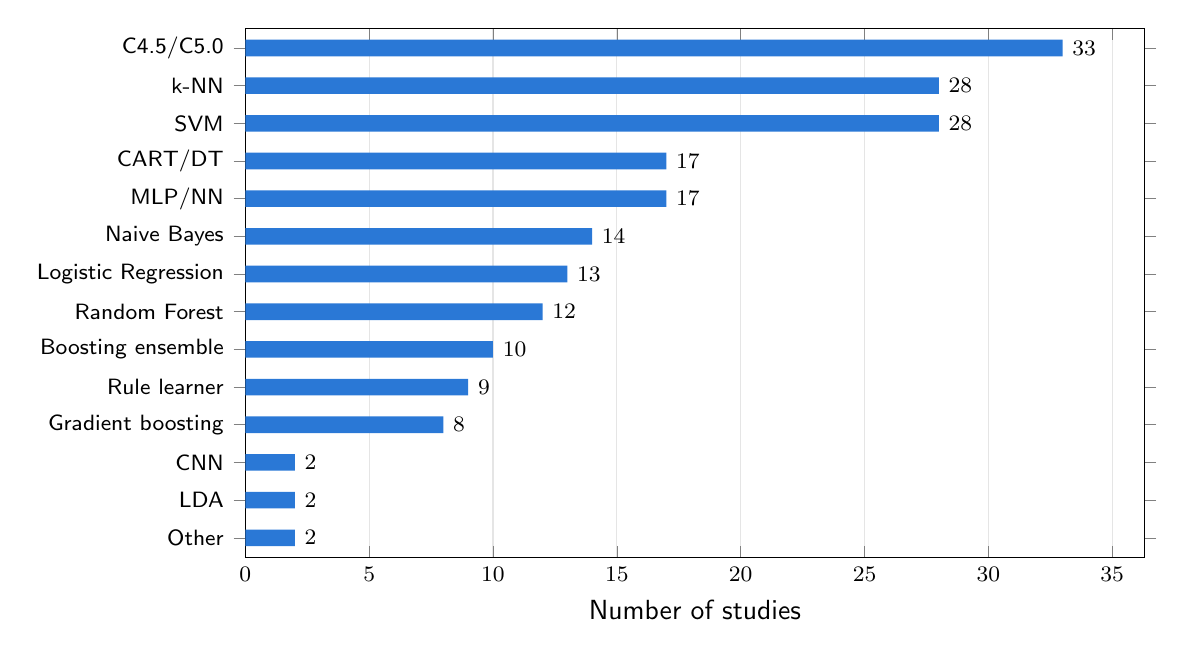
\begin{tikzpicture}
\begin{axis}[xbar,width=13cm,height=8.3cm,bar width=6pt,xmin=0,y dir=reverse,ytick={0,...,13},
  yticklabels={{C4.5/C5.0},{k-NN},{SVM},{CART/DT},{MLP/NN},{Naive Bayes},{Logistic Regression},{Random Forest},{Boosting ensemble},{Rule learner},{Gradient boosting},{CNN},{LDA},{Other}},xlabel={Number of studies},enlarge y limits=0.04,nodes near coords,nodes near coords style={font=\footnotesize},enlarge x limits={upper,value=0.1},
  tick label style={font=\footnotesize},legend cell align=left,legend style={font=\footnotesize,at={(0.98,0.02)},anchor=south east,draw=none},xmajorgrids,grid style={gray!20}]
\addplot[fill=sOne,draw=none] coordinates {(33,0) (28,1) (28,2) (17,3) (17,4) (14,5) (13,6) (12,7) (10,8) (9,9) (8,10) (2,11) (2,12) (2,13)};
\end{axis}
\end{tikzpicture}
\end{document}
